%===========================================================================
%	V. Implementation
%===========================================================================

This chapter accompanies the process of practical implementation of the target solution. It aims to enhance the current solution by means of the task definition (cf. Chapter \ref{sec:1-task}) and the findings from the actual state analysis (cf. Chapter \ref{chap:actual-state-analysis}). Specifically, three main aspects are expected to be added to the solution after implementation, being

\begin{enumerate}
	\item the decapsulation of the analytical scripts from the Apache Airflow instance by means of containerized microservice enablement,
	\item the inclusion of technical DataOps standards, specifically enabled by \acs{iam}, \ac{vcs}, \ac{cicd} and \ac{iac}, and finally
	\item the implementation of the DataOps testing framework (cf. Chapter \ref{chap:testing-framework}).
\end{enumerate}

The order of documentation does not necessarily reflect the implementation sequence of the project. Since this thesis can also be seen as a guideline for future DataOps projects, the implementation steps are provided in order to build on one another in the most useful way. The first two implementation tasks are performed for the entire data pipeline, while DataOps testing is exemplarily implemented for the Conversion Stage.

\section{Server-Less Architecture Enablement}
In order to achieve the goal of a server-less analytics architecture, the current architecture of the Value Pipeline needs to be revisited. Currently, the analysis is directly performed on the Airflow server instance (cf. Section \ref{sec:3-data-pipeline}). Instead, it is desired that each analytical step can be performed and configured independently while also complying to the server-less philosophy. This results in a high-level design change depicted in Figure \ref{fig:5-new-pipeline}.
\newpage

\begin{figure}[h!]
	\centering
	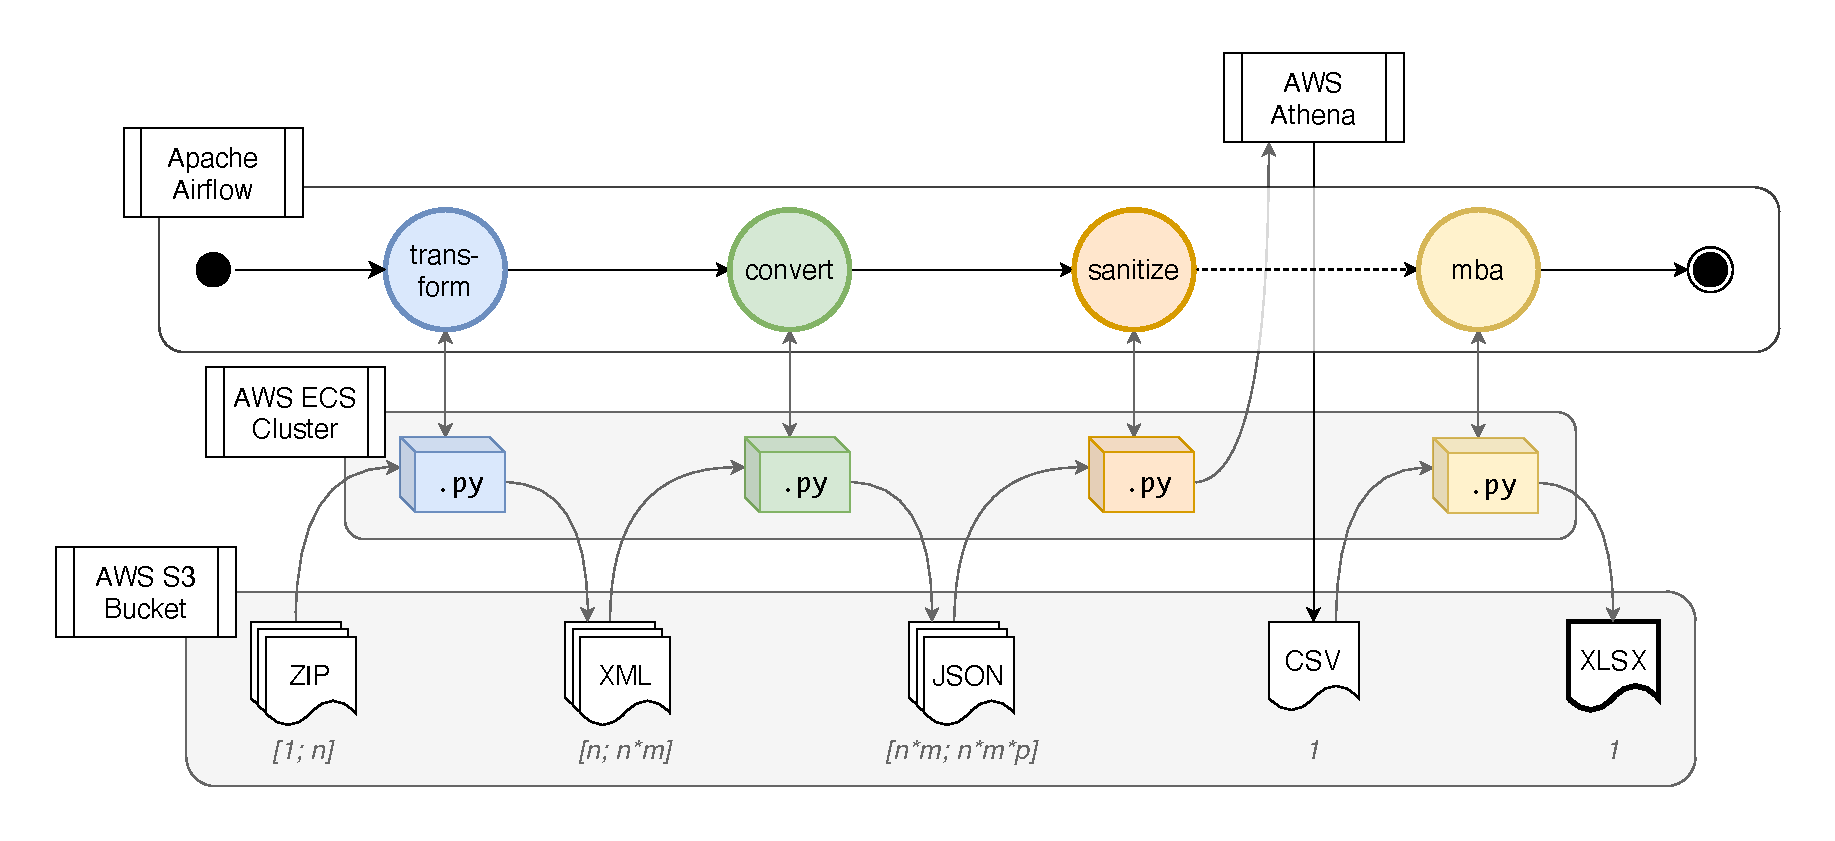
\includegraphics[width=\linewidth]{main-matter/img/5-new-pipeline.pdf}
	\caption{Revisited Data Pipeline Architecture (Server-Less)}
	\label{fig:5-new-pipeline}
\end{figure}

As visualized above, the new architecture outsources the Python analysis scripts out of the Airflow instance. Instead, they create individual microservices now, deployed as virtual containers. These containers, typically realized with the \textit{Docker} containerization software \cite{docker}, contain all required dependencies to run their services. \ac{aws}' \textit{\ac{ecs}} can be used for the server-less deployment and execution of these container tasks \cite{ecs}. With this architecture change, Airflow only remains an orchestration tool that starts the appropriate container tasks. Now, the analytical process is no longer depending on a single virtual server instance. The tasks report their statuses back to Airflow, resulting in Airflow either triggering the next service or terminating the process if an error occurs.

\subsection{Microservice Containerization}
In microservice virtualization, containers are the final desired product. The goal is to have a sequence of commands that encapsulate the Python program code of each individual stage inside their own containers, considering individual stage requirements. To achieve this goal, the intermediate creation of a so-called \textit{image} is required, which provides basic components for making the service runnable \cite{docker}. Before running the container, specific configurations based on the image can been performed.

Docker images are defined by means of a \textit{Dockerfile} \cite{docker}. The tasks inside this file are sequentially executed when creating the image. Exemplarily, the Dockerfile of the Conversion Stage can be seen below.
\newpage
\begin{listing}
	\inputminted{dockerfile}{main-matter/src/5-convert-dockerfile}
	\caption{Dockerfile of the Conversion Stage}
	\label{src:5-convert-dockerfile}
\end{listing}

As can be seen in Source Code Excerpt \ref{src:5-convert-dockerfile}, the image definition begins with referencing the base image (l. 1). This contains a lightweight operating system with the capability of running Python. The Dockerfile also specifies the working directory (l. 2) and prepares environment variables (ll. 4--11) for the container that contain \ac{aws} credentials as well as designated \ac{s3} path \acp{uri} for input and output data locations. The credentials are required for the service to perform its steps on the designated \ac{aws} infrastructure. These environment variables will receive their values during the build process of the container (i.e., when executing the image). This is because such data locations are not expected to remain static for a long period of time. Plus, different data locations have to be provided during the upcoming testing of the containers than during production-grade performance. This data parametrization aids this process. Finally, the local package directory is added to the working directory of the image (l. 16) and all required Python dependencies (for both running and testing) are installed via the \acs{pip} Python package manager (ll. 18--19). These dependencies are specified in the corresponding \texttt{requirements.txt} files inside the package directory.

The environment variables will prove valuable during DataOps enablement. By defining granular \ac{aws} credentials, each stage is only authorized to read and write to their designated \ac{s3} data lake subareas. This creates separated environments for each development stage.

The image can now be build using the \texttt{docker build} command. The design of the Dockerfile requires that the environment variables are passed before container execution (i.e., via arguments in the \texttt{docker build} or \texttt{docker run} command). The image receives a unique tag and the Dockerfile is referenced for correct handling of relative paths. Finally, the image can be used for running the container. This is achieved using the \texttt{docker run} command, specifying which command to run inside the container (e.g., for the Conversion Stage, \texttt{python ./convert.py} for executing the analytics script). This runs the container inside the local system.

\subsection{Image Deployment}
Instead of the container running locally, it is desired to execute it inside the server-less \ac{ecs}. This requires the preliminary deployment to an associated \ac{aws} service, the \textit{\ac{ecr}}. \ac{ecr} is an image repository that is designed to hold different versions of an image \cite{ecr}. This means that each of the four analytics pipeline stages receives its own \ac{ecr}. The image deployment and container execution strategy is depicted in Figure \ref{fig:5-container-deployment} below.

\begin{figure}[h!]
	\centering
	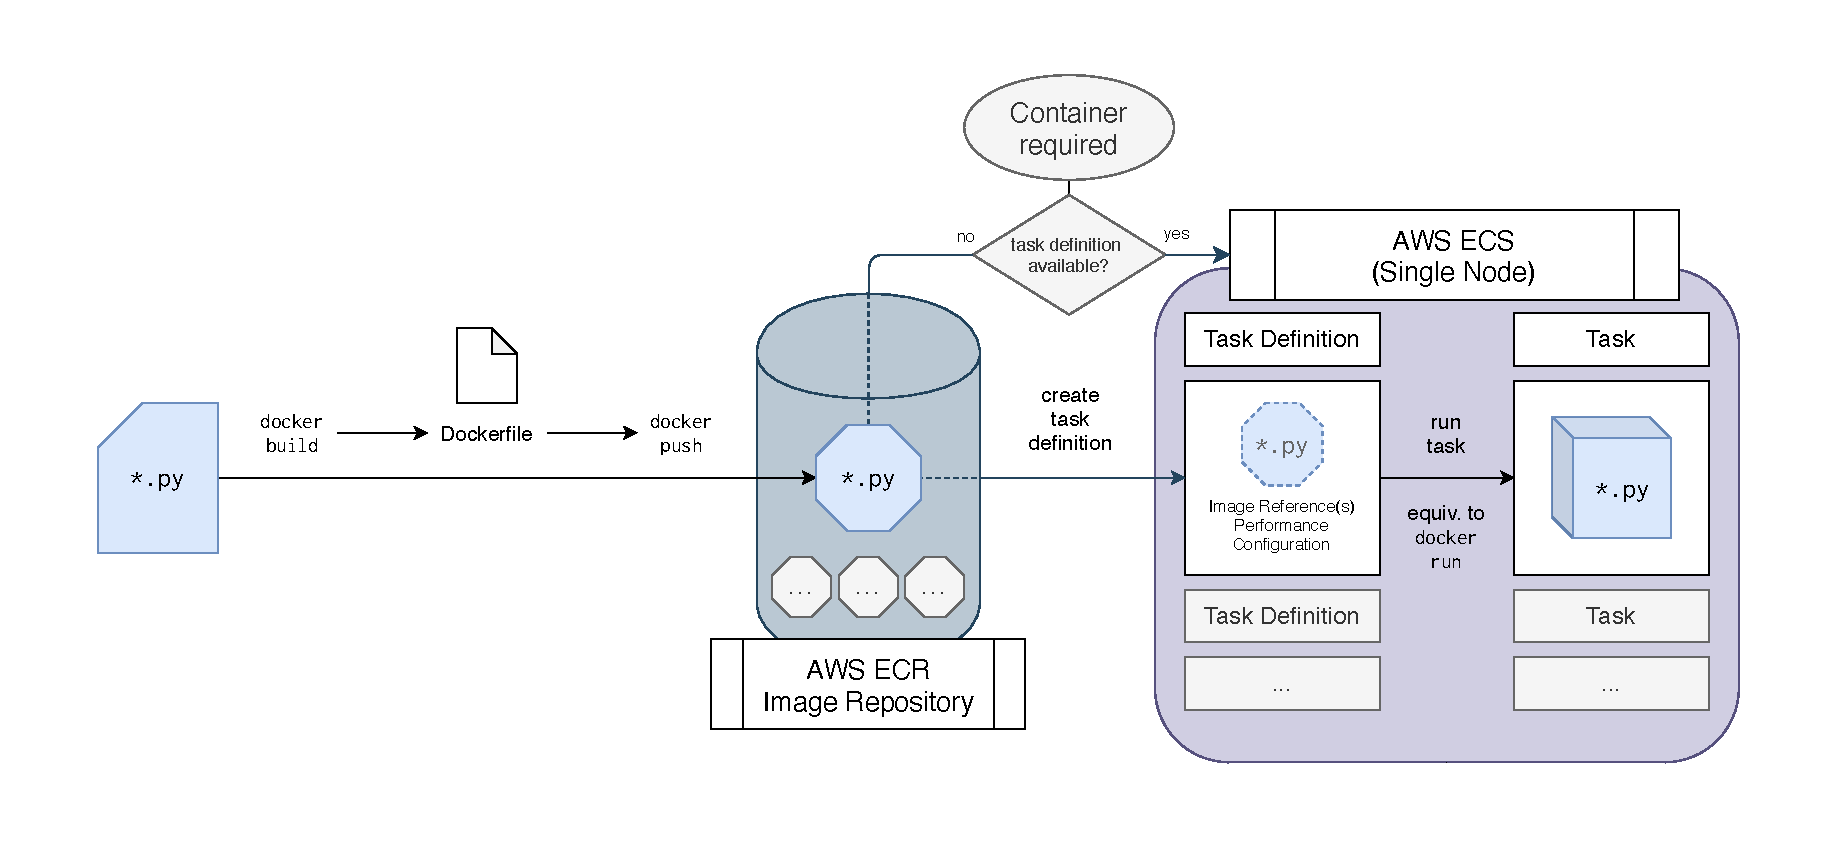
\includegraphics[width=\linewidth]{main-matter/img/5-container-deployment.pdf}
	\caption{Microservice Deployment Process}
	\label{fig:5-container-deployment}	
\end{figure}

Following the flow of the figure, the image is build by means of its Dockerfile and pushed to the designated \ac{ecr}. The octagon shape is used to describe an image. The execution requires another preliminary step which is the task definition of the container. This is because \ac{ecs} can also perform container execution sequences, periodic repetitions of the task, etc. Plus, each task can have different performance requirements. The task definition allows for individual hardware specification (e.g., processing power, memory, etc.) \cite{ecs}. Thus, the task definition can be seen as a blueprint for the (more or less complex) container service. For the data pipeline stages, a task with basic performance specifications as well as one image reference for running the applicable container once, suffices. The task can now be run based on its task definition, providing information on which Python script to run. This executes the task and tears down the container after the task has been worked through or an error has occurred. When the container service is required again and the image repository has not changed, the previous task definition can be directly executed.

\subsection{Server-Less Container Execution via Airflow}
Returning to the high-level overview, creating and running the task definition is performed by Airflow via \texttt{boto3}. The Airflow \ac{dag} controller is redesigned to constantly evaluate the state of \ac{ecr} and \ac{ecs}. It checks for images inside each stage's image repository and builds the applicable task definitions. When all task definitions of all four pipeline stages are present, the Airflow \ac{dag} is ready for execution. The only task inside each individual step of the \ac{dag} is to execute the task definition and evaluate the container response. The \ac{dag} is then executed periodically, e.g. once per day.

Because of the periodic review, the most recent \ac{ecr} images and \ac{ecs} task definition references need to be saved inside Airflow variables to prevent the system from constantly recreating the same task definitions, resulting in an endless loop and, thus, in infrastructure overload.

In case a new version for a stage is recognized, a new task definition is created and re-referenced inside the \ac{dag}, enabling automatic updating of the pipeline solution.

\section{DataOps Enablement}
The next step is to include DataOps-related technologies to the project. They have mostly to do with general solution automation and environment management. Specifically, the following aspects are implemented and configured:

\begin{enumerate}
	\item Enhanced permission management via \acs{aws} \acf{iam},
	\item \acf{vcs} by using \textit{Git} and a \textit{GitHub} repository,
	\item \acf{cicd} by using the \textit{Jenkins} automation software, and
	\item \acf{iac} by using the \textit{Terraform} infrastructure automation tool as well as the \textit{Ansible} infrastructure provisioning software.
\end{enumerate}

These processes will support and build on each other during development for both automation and environment management disciplines.

\subsection{Enhanced Permission Management: \acs{aws} \acs{iam} Roles}
\acs{aws} \acs{iam} roles are used to provide different access permissions to different users and resources. If a user or resource tries to perform actions on \ac{aws} services (e.g., via \acs{cli} or \acs{api}), the system checks if the required credentials are present to perform this action. The credentials are provided in the form of asynchronous encryption, resulting in a public \textit{Access Key ID} and in a private \textit{Secret Access Key} \cite{iam}.

Because of the static nature of the current solution, only one full-access \ac{iam} role is used. This is not desirable from multiple perspectives. Each developer should be provided an \ac{iam} role that is sufficient for his or her needs. The underlying permissions should not exceed these needs in order to prevent collision or changes within \ac{aws} resources outside of the scope of the developer. The same aspect applies to resources that automatically perform actions on other resources. Another important factor is data privacy. In a production-grade environment with sensitive data, it is crucial and binding by law that the data is only seen and processed by authorized entities. 

For instance, if a data pipeline stage is misconfigured and tries to read from another area of the \ac{s3} data lake, the process will terminate when the given \ac{iam} role prohibits this action. Otherwise, the stage would be granted access to data that is not required for its task. In that case, correctly configured \ac{iam} roles can also prevent errors in case the content of the incorrect \ac{s3} area cannot be processed by the current analytics stage.

Considering the \ac{mba} data pipeline, the present variety of resources requires different permissions on a number of other different resources. Table \ref{tab:5-iam} describes all permissions required by different components.

\begin{table}[h!]
	\centering
	\begin{tabular}{r!{\vrule width 1pt}l|l|l}
\textbf{Component}                                  & \textbf{Resource}         & \textbf{Type} & \textbf{Scope}              \\ \ChangeRT{1pt}
\multirow{2}{*}{Airflow}                            & \ac{ecr} & Full Access   & designated stage image repositories          \\ \cline{2-4}
                                                    & \ac{ecs} & Full Access   & designated container service                 \\	 \ChangeRT{1pt}
\multicolumn{4}{c}{\textbf{Stages}}                                                                                           \\ \ChangeRT{1pt}
\multirow{2}{*}{\textbf{Transformation}}            & \ac{s3}  & Read          & \texttt{./landing/}      				  \\ \cline{2-4}
                                                    & \ac{s3}  & Write         & \texttt{./**/raw/}       				  \\ \hline
\multirow{2}{*}{\textbf{Conversion}}                & \ac{s3}  & Read          & \texttt{./**/raw/}       			  	  \\ \cline{2-4}
                                                    & \ac{s3}  & Write         & \texttt{./**/converted/} 				  \\ \hline
\multirow{3}{*}{\textbf{Sanitization}}              & Athena   & Full Access   & designated database                          \\ \cline{2-4}
                                                    & \ac{s3}  & Read          & \texttt{./**/converted/} 				  \\ \cline{2-4}
                                                    & \ac{s3}  & Write         & \texttt{./**/sanitized/} 				  \\ \hline
\multirow{2}{*}{\textbf{\ac{mba}}} 					& \ac{s3}  & Read          & \texttt{./**/sanitized/}  				  \\ \cline{2-4}
                                                    & \ac{s3}  & Write         & \texttt{./**/}          
\end{tabular}
	\caption{\acs{aws} \acs{iam} Role Overview}
	\label{tab:5-iam}
\end{table}

Each data lake scope begins with \texttt{s3://datalake}, specifying the same \ac{s3} bucket for every component. This information is omitted in Table \ref{tab:5-iam} for simplicity reasons. The \texttt{**} symbols represent a wildcard that allow for accessing the different job areas of the data lake. These roles are setup within the \ac{aws} \ac{iam} Console and passed to the individual components as environment variables \cite{iam}, depending on their individual deployment. 

\subsection{\acs{vcs} Enablement: \textit{Git} and \textit{GitHub}}
Embedding the project inside a \ac{vcs} allows for collaborative development. When working with such a system, the common codebase is located inside a distributed repository. This repository can be cloned (i.e., copied) to the developers local development environment. \textit{Committing} to feature \textit{branches} (i.e., performing and saving changes of the personal version of ones source code) does not collide with the source code versions of other developers \cite[9\psqq]{Chacon2020}. Plus, since the project at hand relies on external programming and developing dependencies (e.g., Python packages and libraries, environment configuration processes, etc.), the repository can also contain configuration utilities for setting up the development sandbox.

\subsubsection{Repository Structure}
A cloned repository is a typical project directory. The repository for the \ac{mba} data pipeline solution looks as follows:
\newpage
\begin{figure}[h!]
	\centering
	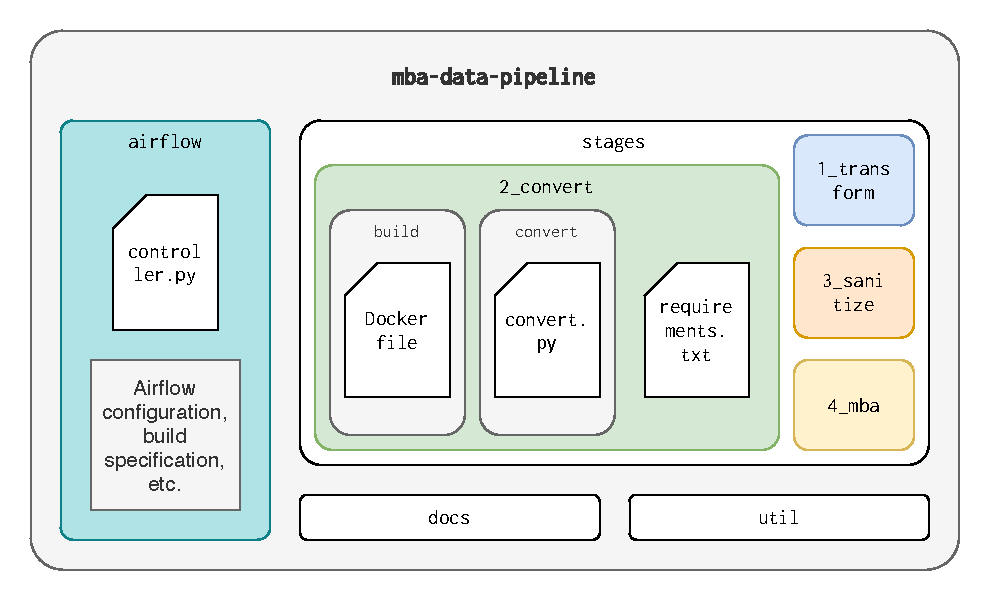
\includegraphics[width=\linewidth]{main-matter/img/5-repo-structure.pdf}
	\caption{Initial Project Repository Structure}
	\label{fig:5-repo-structure}
\end{figure}

The repository presented in Figure \ref{fig:5-repo-structure} is a so-called \textit{monolithic} repository. Since the project is expected to be developed by separate stage teams, this repository de facto consists of multiple projects. Starting at the root of the directory, the repository contains subdirectories for Airflow pipeline management, the individual stages of the data pipeline, documentation as well as miscellaneous utilities. The Airflow pipeline management consists of the pipeline controller script, as well as supporting build files that are outside the scope of this thesis. More importantly, the individual stages are, again, divided into subdirectories. Each stage has its own build directory (currently including its Dockerfile), a package directory (currently including all productive source code), as well as dedicated requirements files required by the source code.

\subsubsection{Repository Setup}
The goal is to create a GitHub repository for the \ac{mba} data pipeline project. First, the project needs to become a Git repository, enabling the version control capability. GitHub is used for the distribution and collaborative management of the code base \cite[25\psqq]{Chacon2020}\cite{github}. First, the project directory needs to be initialized by means of Git. Then, the repository can be created within the GitHub web \ac{ui}. Lastly, the local Git repository is pushed to the recently created GitHub repository.

In order to allow for the automatic configuration of development sandboxes, each stage directory receives a \textit{Makefile} that creates shortcuts for configuration commands. This includes local building and executing of a Docker container. Other development conventions (e.g., for Python, that development should be conducted in Python \textit{virtual environments}), cannot be enforced but only suggested within the project documentation.

\subsubsection{Branching Strategy}
Currently, an authorized developer is able to clone this repository, make any kind of changes, and push these changes back to the repository. This kind of workflow is not desired which is why \textit{branching} is introduced. Branching is a GitHub feature that supports development environment management within the repository \cite[62\psqq]{Chacon2020}. At this point, only one branch, the \texttt{master} branch, exists. It holds the history of all versions of the source code. These versions change when updated code is pushed to the brach. In practice, the \texttt{master} branch is supposed to be the communal \textit{single version of the truth}. It is expected to be runnable and should reflect the source code of the solution which is currently used in production. When changes of all sorts are possible inside the \texttt{master} branch, the validity of it gets lost. This is why this branch needs to be protected such that only evaluated changes can be pushed to this area of the repository.

Branching is a matter of project convention definition. The general goal is that on-going development of an arbitrary feature is conducted outside of the \texttt{master} branch (i.e., on separated feature branches). Each (sub-)team working on an individual feature \textit{branches} from the \texttt{master} branch, resulting in an exact copy of its origin in the beginning. All changes pushed to the new branch do not affect the \textit{master} brach. When the feature is considered done, a GitHub \textit{pull request} is created \cite{github}. This pull request is evaluated based on its configuration. If the evaluation passes, the feature branch gets \textit{merged} with the \texttt{master} branch, meaning that all changes are applied to the source code inside the \texttt{master} branch at once. Finally, the feature branch is deleted. From now on, the updated \texttt{master} branch is used as the starting point for further development. This branching workflow is commonly referred to as the \textit{GitHub Flow} \cite{GitHub2020}, depicted in Figure \ref{fig:5-github-flow}.
\newpage
\begin{figure}[h!]
	\centering
	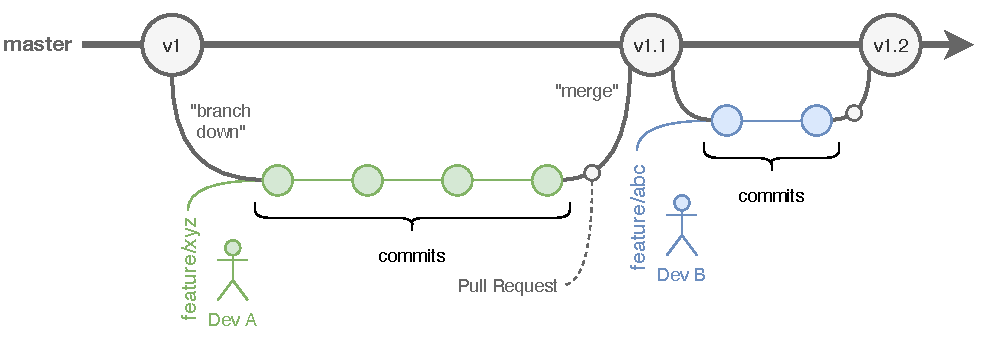
\includegraphics[width=\linewidth]{main-matter/img/5-github-flow.pdf}
	\caption[\textit{GitHub Flow} Branching Strategy]{\textit{GitHub Flow} Branching Strategy (per \cite{GitHub2020})}
	\label{fig:5-github-flow}
\end{figure}

The branching strategy, as presented above, is typical for a fast-paced development cycle. Each approved change, no matter how small, is directly published into production. Apart from that, other branching strategies could be applied. It might be reasonable to include separate \texttt{development} and \texttt{release} branches. The \texttt{development} branch could become the starting point for new features and could contain features that have not been published yet. In case of a slower release cycle, the development branch could be merged with the \textit{release} branch for compatibility testing purposes and deployed into production (i.e., merged with the \texttt{master} branch) afterwards. Another \texttt{hotfix} branch might be used for quick bug fixes that branches from the \textit{master} branch, fixes the bug, and merges back into production \cite{Driessen2010}.

For the sake of simplicity and demonstrability, the former described branching strategy is chosen for the \ac{mba} data pipeline. The \texttt{master} branch is configured inside GitHub to only accept pull requests for incoming changes, not direct pushed onto the \texttt{master} branch. Later, the pull request functionality will be enriched with \ac{cicd}. In case the process runs through without errors, the changes are evaluated positively and cleared for the merging process.

\subsection{\acs{cicd} Enablement: \textit{Jenkins}}
\ac{cicd} is expected to enhance and automate two aspects inside the development process of the \ac{mba} data pipeline solution:
\begin{enumerate}
	\item It handles the build and deployment of virtual Docker images and containers by means of Figure \ref{fig:5-container-deployment}. This also includes providing each task with its designated environment variables for infrastructure access as well as analytics data input and output locations.
	\item It automates the execution and reporting of test cases, only allowing for approved deployment of tested versions of the solution. This process supports the previously mentioned pull requests which will fail when tests are evaluated negatively.
\end{enumerate}

The latter aspect will be implemented in Section \ref{sec:5-testing-implementation}.

The desired DataOps \ac{cicd} workflow is depicted in Figure \ref{fig:5-cicd}. It considers testing a black box for now. It is noteworthy to mention that each stage of the data pipeline could have different requirements for its deployment, which is why each stage receives its own \ac{cicd} pipeline. This becomes clear when considering testing since each stage performs different tasks and requires different test cases.

\begin{figure}[h!]
	\centering
	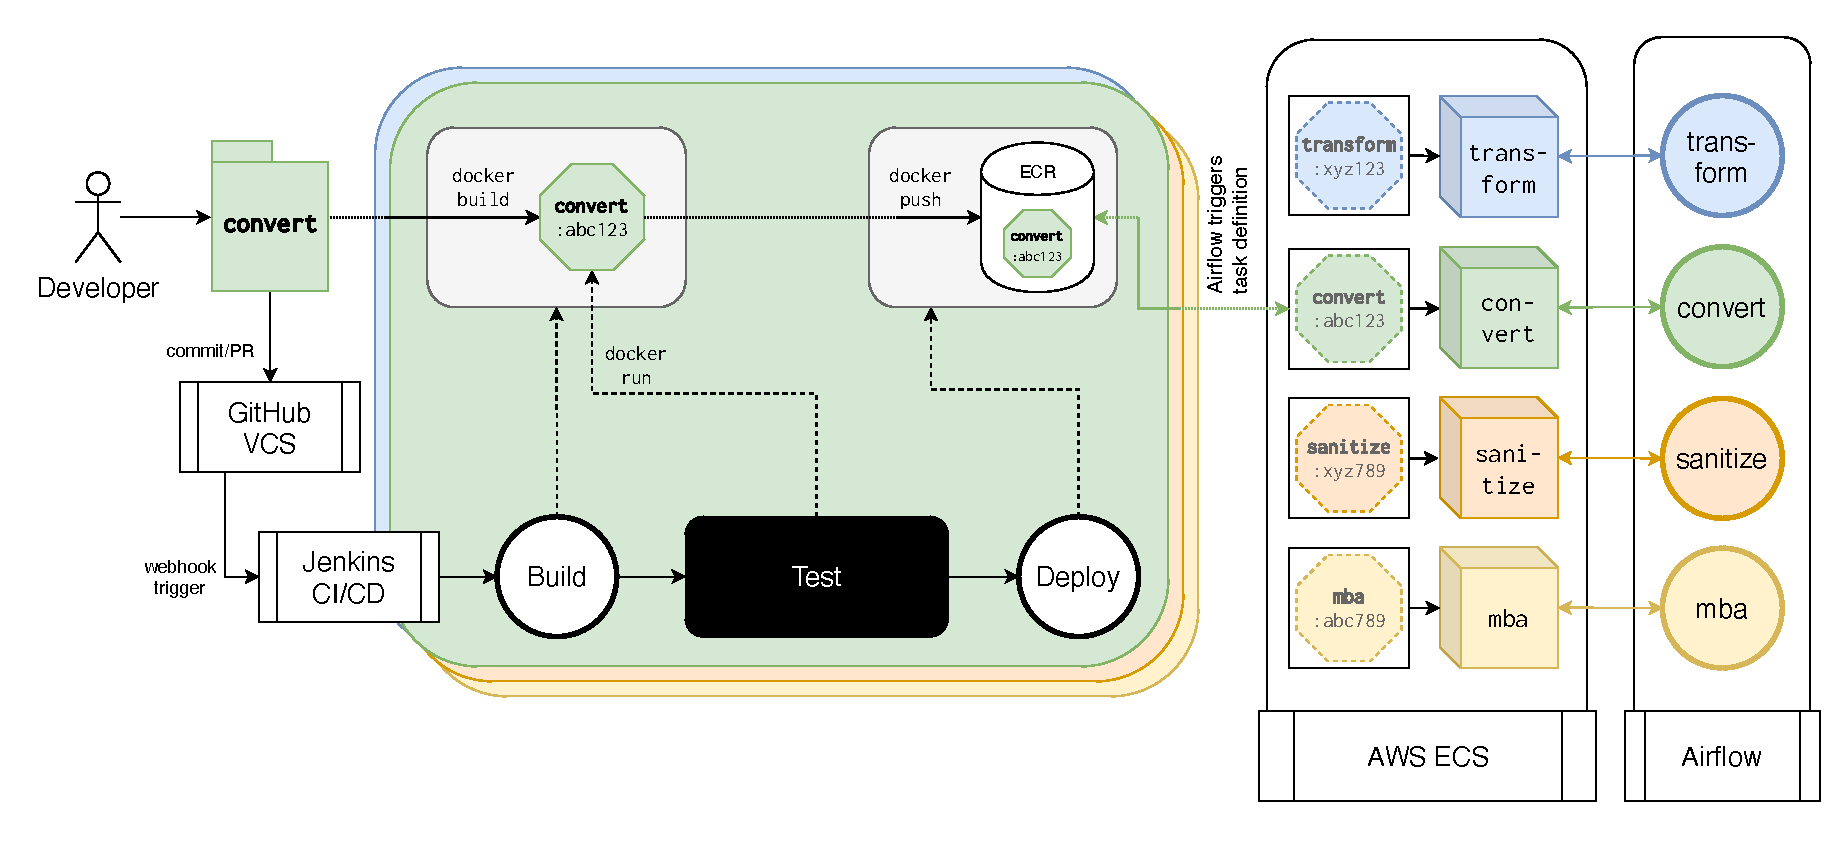
\includegraphics[width=\linewidth]{main-matter/img/5-cicd.pdf}
	\caption{DataOps \acs{cicd} Architecture for the Conversion Stage}
	\label{fig:5-cicd}
\end{figure}

Figure \ref{fig:5-cicd} represents the \ac{cicd} workflow of the Conversion Stage. It is meant to be executed whenever a GitHub pull request of a Conversion Stage-related feature is opened. This pull request appearance should trigger the corresponding pipeline, realized with the \textit{Jenkins} \ac{cicd} software \cite{jenkins}. The first step needs to build a virtual Docker image using the target source code files from the pull request. Again, this build process is done by means of the stage's specific Dockerfile and requires additional arguments for the containers environment variables. When the image is built, the build stage of the \ac{cicd} pipeline is completed. Later, this this image will be run on the Jenkins instance for different testing purposes. After these tests pass, the image is ready for deployment. Airflow expects runnable images inside their designated \ac{ecr} repositories which is why the image, individually tagged, is pushed to its repository. The deployment process is done at this point. When Airflow needs to run a new analysis, the controller script will scan the registry for the latest image, recognize a new image, create the applicable task definition and run the container based on the newly deployed image. Every further analysis will be done utilizing this image until a new image is deployed again.

\subsubsection{Jenkins Software and Pipeline Setup}
Comparable to Apache Airflow, Jenkins needs to be considered as an external application that needs to reside on some kind of infrastructure. For efficiency reasons, the \ac{ec2} instance already running Airflow also receives Jenkins. Both web servers now run simultaneously on different ports for \acs{http} access.

Jenkins provides different blueprints for \ac{cicd} pipelines. The DataOps \ac{cicd} pipeline of the \ac{mba} data pipeline needs to recognize pull requests that originate from different feature branches within GitHub. This is why the \textit{Multibranch Pipeline} is chosen \cite{jenkins}. Such a pipeline is created for each of the four stages of the data pipeline. The branch needs to be granted access to the GitHub repository. Since the project is working with a monolithic repository, each \ac{cicd} pipeline needs to be configured in such a way that it only recognized changes and pull requests to specific areas of the repository.

There are multiple ways to achieve this configuration. Jenkins distinguished between branches and pull requests, meaning that a branch with a pending pull request is listed and evaluated by Jenkins \textit{twice}. Jenkins is therefore configured to disregard branches that are also filed as pull requests. The only non-pull request branch should be the \texttt{master} brach since all other branches are expected to be in development if no pull request is present. Thus, Jenkins should only consider \texttt{master} a long-lasting branch. The pipeline should only consider stage-specific changes, which is why Jenkins should filter each pull request by its GitHub label. This requires the developer to add the specific stage label when filing a pull request. Finally, Jenkins should automatically run a \ac{cicd} job inside the corresponding pipeline when a change is recognized. This needs to be enabled in both Jenkins and GitHub. GitHub needs to send a \texttt{POST} request to Jenkins when a pull request is filed, whereas Jenkins needs to trigger the corresponding pipeline on \texttt{POST} request arrival.

\subsubsection{Jenkins Credential Management}
The virtual microservices need to receive their \ac{aws} \ac{iam} access credentials during their build process. Since this process is expected to be covered by \ac{cicd}, Jenkins needs to hold these credentials and pass these to the corresponding stage containers inside its \ac{cicd} pipeline workflow. This is achieved by adding the individual credentials to Jenkins' encrypted credential storage \cite{jenkins}. These need to include all stage-related credential key-value pairs that provide appropriate access to the analytics resources as described in Table \ref{tab:5-iam}. Additionally, Jenkins needs to be granted permission to push images to the \ac{ecr} repositories. The corresponding credential should not be mistaken with a separate \ac{iam} role. Rather, Jenkins needs to hold a login token for \ac{ecr} that is retrieved via \ac{aws} \acs{cli} \cite{ecr}. This process is identical to other Docker registry services, independent from the actual vendor.

Jenkins will then pass the encrypted credentials to the corresponding pipelines \cite{ecr}, resulting in no hard-coded credentials in any configuration file.

\subsubsection{Pipeline Workflow Declaration}
After the pipeline preferences have been configured, the actual pipeline workflow needs to be declared for each stage. In Jenkins, this is done via a so-called \textit{Jenkinsfile}. It is written in \textit{Groovy} programming language and contains instructions for each stage of the pipeline \cite{jenkins}. A sample Jenkinsfile for the Conversion Stage is shown below.

\begin{listing}[h!]
	\inputminted{groovy}{main-matter/src/5-jenkinsfile-build}
	\caption{Jenkinsfile Build Stage for the Conversion Stage}
	\label{src:5-jenkinsfile-build}
\end{listing}

Source Code Excerpt \ref{src:5-jenkinsfile-build} shows the build stage inside the Jenkinsfile. It retrieves the corresponding stage credentials from Jenkins' credential storage (ll. 8--11) and executes the build process of the Docker image (ll. 12--19). The image needs to be tagged in an \ac{aws}-provided \ac{ecr} format such that it is assigned to the correct repository during the deployment phase. This tag includes the corresponding Git commit ID for versioning purposes (l. 14) which is passed to Jenkins by the previously mentioned GitHub \texttt{POST} request trigger. Prior to the build, the arguments for the \ac{aws} \ac{iam} credential pair are passed (ll. 15--16) and set as environment variables by means of the Dockerfile specification. Later, the remaining arguments for input and output data locations will be covered by Airflow when calling for a new analytics job. Finally, the Dockerfile (l. 17) and the build context for relative path recognition (l. 18) are specified. This command is executed by the Jenkins \ac{cicd} pipeline job. In case of a correct execution, the next stage is performed. Since testing is omitted for now, it directly continues with the deployment, shown below. 

\begin{listing}[h!]
	\inputminted{groovy}{main-matter/src/5-jenkinsfile-deploy}
	\caption{Jenkinsfile Deployment Stage for the Conversion Stage}
	\label{src:5-jenkinsfile-deploy}
\end{listing}

Source Code Excerpt \ref{src:5-jenkinsfile-deploy} shows the deployment stage inside the Jenkinsfile. It retrieves the \ac{ecr} credentials (ll. 11--13) and performs the image deployment via \texttt{docker push} (ll. 14--17). This action is performed for two tags: the commit ID for versioning and the conventional \texttt{latest} tag such that Airflow recognizes it as the most recent, production-ready image. \\\

All in all, the current \ac{cicd} solution builds and deploys a new version into production when a feature pull request is filed to GitHub. Airflow recognizes the change based on its controller script and uses the new image for the corresponding stage for container execution and evaluation.

\subsection{\acs{iac} Enablement: \textit{Terraform} and \textit{Ansible}}
Another form of automation that is part of DataOps is automatic infrastructure deployment via \ac{iac}. The project at hand requires a variety of different \ac{aws} infrastructural resources, including the effort of configuration. In case that the infrastructure needs to be setup inside a different \ac{aws} account or it breaks during development, it is not desirable to be forced to start building up the infrastructure from scratch. Instead, the following \ac{iac} architecture is proposed.

\begin{figure}[h!]
	\centering
	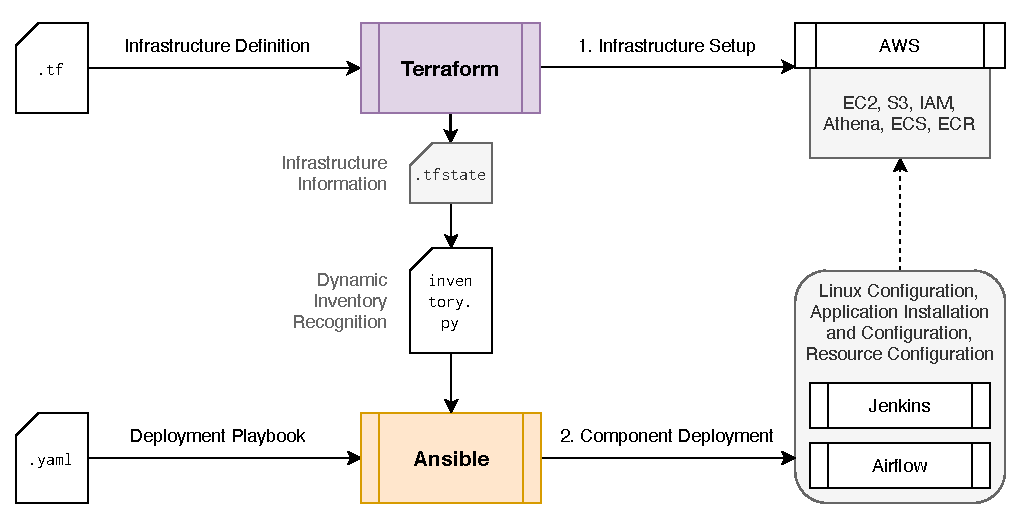
\includegraphics[width=\linewidth]{main-matter/img/5-iac}
	\caption{\acs{iac} Infrastructure Deployment Strategy}
	\label{fig:5-iac}
\end{figure}

The \ac{iac} architecture, visualized in Figure \ref{fig:5-iac}, is made out of two steps. First, all required \ac{aws} services are defined for the \textit{Terraform} infrastructure provisioning tool. This also includes basic configuration of networking and access management. In general, all configuration that can be done via the web \acs{ui}-based \ac{aws} Console or the \ac{aws} \acs{cli} or \acs{api} can be done via Terraform. Terraform requires an individual \ac{iam} role that allows it to create the infrastructure. When the deployment script is performed via the Terraform \acs{cli}, it creates a \texttt{.tfstate} file in \ac{json} format \cite{terraform}, summarizing all created infrastructure including public IP addresses, infrastructure IDs, etc.

This infrastructure needs to be configured via the \textit{Ansible} infrastructure orchestration software. This includes the Linux configuration of the \ac{ec2} instance, the creation of \ac{s3} data lake (sub-)areas, etc. Basically, the goal is to run the corresponding commands for Terraform and Ansible, resulting in an up-and-running infrastructure, ready for production-grade usage.

Ansible requires an intermediate step before being able to perform actions on the infrastructure, which is the recognition of the resource inventory. This can be done manually, which is not desired, or via a dynamic inventory recognition script. This makes use of the previously generated \texttt{.tfstate} file and provides Ansible with information and access to the respective infrastructure. Then, so-called Ansible \textit{Playbooks} are written and executed. These hold tasks for the configuration, platform and application installation, etc. \cite{ansible}. Most importantly, Ansible is in charge of installing and configuring Airflow and Jenkins. Airflow is installed and receives its controller script as well as further configuration from the project repository. Jenkins is installed, pre-configured, and required plugins are installed. 

Unfortunately, these applications do not provide all necessary Ansible endpoints. This means that not all configuration steps can be done automatically but require manual adjustment. This includes Jenkins credential management, pipeline creation, etc. All in all, the infrastructure automation is valuable nonetheless since the manual setup process is significantly reduced.

\section{Testing Framework Implementation} \label{sec:5-testing-implementation}
At this point, the DataOps capability of the \ac{mba} pipeline solution is sufficient to be enhanced by means of the testing framework, designed in Chapter \ref{chap:testing-framework}. The practical implementation of the framework goes hand-in-hand with its design steps.
\begin{enumerate}
	\item The data event handling mechanisms need to be implemented inside the productive analytics solution.
	\item The test data (suites) need to be provisioned inside a separated data environment.
	\item DataOps solution tests need to be written and executed by the Jenkins pipeline, making use of the available test data. The test outcome evaluation inside Jenkins will decide if the given version update may be deployed into production.
\end{enumerate}

\subsection{Data Event Handling Implementation}
In general, the goal is that the data event handling inside the solution complies with its corresponding definition. When summarizing all event handling processes by means of their actions, the following capabilities need to be ensured:

\begin{itemize}
	\item Logging of different event severities.
	\item Process termination for \texttt{CRITICAL} events.
	\item Threshold adjustment and evaluation for \texttt{ERROR} and \texttt{WARNING} events.
	\item Dynamic File Flagging for \texttt{ERROR} and \texttt{WARNING} events.
\end{itemize}

Again, there are multiple ways to achieve this kind of data handling capability in practice. In order to keep the productive analytics source code readable and maintainable, data handling is outsourced to its own class \texttt{DataHandling} that is instantiated inside the solution. It receives the references to the data in question, threshold limits, etc. during initialization. Each data event definition receives its own function which is then called by the solution at the appropriate point during its runtime. The visualization of the Conversion Stage, including all its data event handlers, can be found in Appendix Figure \ref{app:new-convert}.

For the sake of clarity, the following paragraphs elaborate on the implementation of the list of general features inside the \texttt{DataHandling} class before presenting exemplary implementations of several data handling functions.

\subsubsection{Event Logging}
Event logging in Python can be realized with Python's standard \texttt{logging} library. The default log severities \texttt{INFO}, \texttt{WARNING}, \texttt{ERROR}, and \texttt{CRITICAL} correspond with the event severities of the testing framework. The \texttt{logging} object is instantiated inside the \texttt{DataHandling} class and configured to write log occurrences of severity \texttt{INFO} and above to a specified file which receives the name of the current analytics job. Each time a log is required, the \texttt{logging} object is called with the message and arguments to be contained.

\subsubsection{Process Termination}
The analytical process needs to be terminated whenever an event of \texttt{CRITICAL} severity occurs. In order to provide helpful monitoring information, the termination should not just shut down the process. Instead, it should prompt a message on why the process needed to be terminated. On the one hand, this is included to the log file by means of the previous section. On the other hand, each critical event receives its own custom Python \textit{Exception}. This exception contains are log-like information message as well as a traceback to the origin of the exception, and hence, termination. This is expected to allow for better understanding and recovery from the underlying issue.

\subsubsection{Thresholding Capability}
As previously mentioned, the threshold percentages are passed to the \texttt{DataHandling} class during initialization. Currently, a value of $0.05$ for \texttt{ERROR} events and $0.1$ for \texttt{WARNING} events, is utilized. This means that five percent of the input data may invoke \texttt{ERROR}s and ten percent of the data may invoke \texttt{WARNING}s. The solution does not take files with multiple data issues into account differently. Eventually, the most severe event is counted for threshold evaluation. At the end of the input data event handling process, the threshold values are evaluated. The process terminates when either one of the thresholds is exceeded. As previously described, transformation and output data is not subject to threshold evaluation but results in instant termination in case an event is invoked (cf. Section \ref{sec:4-1-4}).

\subsubsection{File Flagging}
\texttt{WARNING} and \texttt{ERROR} events additionally flag files by means of their invocation event. The \ac{aws} Python \ac{sdk} \texttt{boto3} is used for this matter since all data resides inside the \ac{s3} data lake. File flagging is implemented inside its own function which is called with the appropriate file reference (i.e., the file to be tagged) and the tag itself. \texttt{boto3} then requests all current tags for the file. In case the tag in question has not been set, it is added to the file now. The tagging information is provided inside the log file with \texttt{INFO} log severity.
\newpage
\subsubsection{Event Handling Implementation Examples}
Now that the components of the event handing are defined, the individual handling functions can be implemented. The following examples go by the data event examples provided in Section \ref{sec:4-1-3-a}, \ref{sec:4-1-3-b}, and \ref{sec:4-1-3-c}.

\paragraph{Example A: Data Source Empty}
\begin{listing}[h!]
	\inputminted{python}{main-matter/src/5-a.py}
	\caption{Implementation of Data Event Example A: Data Source Empty}
	\label{src:5-example-a-implementation}
\end{listing}
Source Code Excerpt \ref{src:5-example-a-implementation} implements the data event handling for an empty data source. The function receives the file references as a parameter (l. 1) and makes use of a \textit{guard} statement to rule out an empty data source first (l. 2). In case this condition does not apply, the function logs the \texttt{CRITICAL} event to the log file, providing information on the \ac{s3} bucket and bucket directory in question (ll. 4--8). These have been passed to the class instance during initialization. At the end, it raises the custom \texttt{S3EmptyError} exception that terminates the process. The exception is prompted, again, with bucket and directory information (l. 9) for improved troubleshooting.
\newpage
\paragraph{Example B: XML File(s) Corrupted}
\begin{listing}[h!]
	\inputminted{python}{main-matter/src/5-b.py}
	\caption{Implementation of Data Event Example B: \acs{xml} File(s) Corrupted}
	\label{src:5-example-b-implementation}
\end{listing}
Source Code Excerpt \ref{src:5-example-b-implementation} implements the data event handling for corrupted \ac{xml} files. Again, the corresponding function receives file references. Since there is a possibility that other \texttt{ERROR} events have already occurred and removed faulty input data, the function checks if there are any files left for evaluation (l. 2). Then, it loops through all files in question and attempts to parse their binary content to \ac{xml} (ll. 6--7). The function makes use of the Python \ac{xml} \texttt{ElementTree} sub-library (initialized as \texttt{et}). By design, the parser function raises an \texttt{ParseError} exception if the data is corrupted. By catching this library exception, the specific data handling can be processed. The log file receives a new line containing the corresponding file information (ll. 9-11). Additionally, the log also mentions that the file in question is skipped because of the \texttt{ERROR} event severity. The file name reference is added to another list that contains all corrupted files (l. 4 and 13) and the error file counter is incremented (l. 14). This will later be used for threshold evaluation. Finally, all corrupted files are removed from the original file reference dictionary (l. 15--16).
\newpage
\paragraph{Example C: Missing Optional Attributes}
\begin{listing}[h!]
	\inputminted{python}{main-matter/src/5-c.py}
	\caption{Implementation of Data Event Example C: XML File(s) Corrupted}
	\label{src:5-example-c-implementation}
\end{listing}
Source Code Excerpt \ref{src:5-example-c-implementation} implements the overall data event handling for missing global attributes. Since the event in question only covers the missing \textit{optional} attributes, the handling of required attributes is omitted here (l. 6). At this point of the analysis, the binary \ac{xml} data has already been parsed to Python standard dictionaries, which is why the function received a dictionary of all \ac{pos} dictionaries (l. 1) and loops over the root dictionary (l. 2). As with the first example, a guard statement is used to rule out the case of any missing argument (ll. 3--4). Then, the keys of the content dictionary are evaluated against the constant class list of optional attributes (ll. 8--10). In case this evaluation results in arguments missing, a list of missing attributes is created (ll. 11-13) and logged alongside the input file name (ll. 14--20). Since this is an event of \texttt{WARNING} severity, the \texttt{WARNING} event file counter is incremented (l. 21) and evaluated at the end of input data event handling. Finally, the source data tagged via the custom tagging function (ll. 22-26)

All further data events are implemented in a similar manner.

\subsection{Test Data Provisioning}
In order to test for correct data handling, appropriate test data is required to invoke the corresponding events. The design of the test data suited of various complexity degrees and use cases has been conducted in Section \ref{sec:4-test-data-design}. The goal now is to provision these suites in order for the planned, holistic DataOps testing integration. Specifically, the test data needs to be available for continuous testing in every phase of development. Since a centralized data lake already exists, the goal can be achieved by adding the test data to the data lake.

\subsubsection{Data Lake Architecture Revision}
The current architecture of the data lake only considers production-grade analytics processes. Simply adding the test data inside this critical environment could be prone to compatibility and analytics correctness issues. Plus, it goes against the DataOps principle of distinct environments. This is why the following data lake architecture revision is proposed:

\begin{figure}[h!]
	\centering
	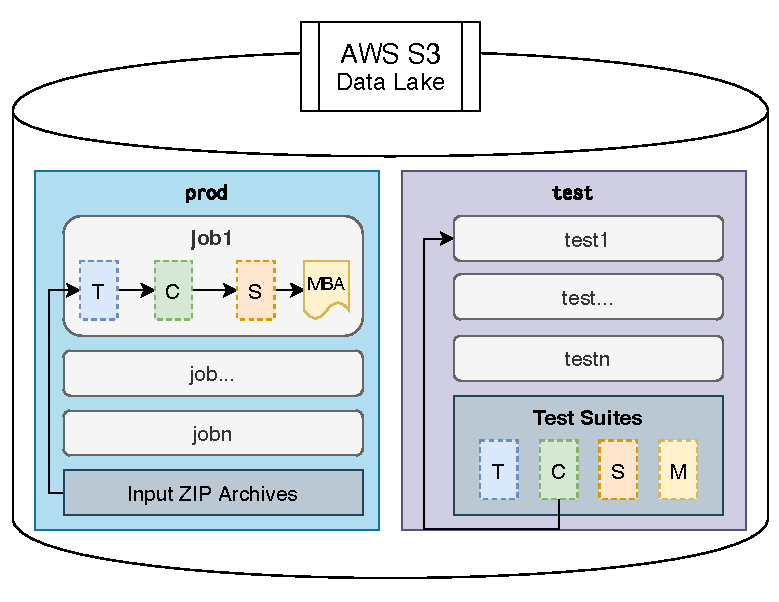
\includegraphics[width=0.67\linewidth]{main-matter/img/5-data-lake-new}
	\caption{Data Lake Architecture Revision}
	\label{fig:5-new-data-lake}
\end{figure}

In the new structure, presented in Figure \ref{fig:5-new-data-lake}, the data lake is environmentally divided at the topmost level. One environment remains the otherwise unchanged production-grade environment, containing raw input data as well as all analytics job subareas. The new testing environment now contains input data test suites for every stage of the pipeline. Since this data is also expected to be processed by the corresponding stage during testing, the area has also got job subareas for each conducted test.
\newpage
With this change, the stages do not conduct test-grade analysis with production-grade data, but remain in a separated testing environment. The corresponding \ac{s3} \acp{uri}, containing test data, are passed to the individual stages. In case all future tests pass, the stages are permitted to receive the production-grade data locations afterwards.

\subsubsection{\acs{iam} Role Revision}
With new environments, new \ac{aws} \ac{iam} roles are required. This maintains another layer of analytical integrity. In case a test stage receives production-grade data references, a correctly configured \ac{iam} role prevents it from performing. Developer sandboxes and their \ac{iam} roles can also be changed here such that the personal environment does not have access to potentially sensitive data.

In practice, each stage receives a second \ac{iam} role for testing purposes. The corresponding credentials are passed as environment variables to the virtual stage container and replaced with the production-grade access credentials after the tests have passed. \\\

With this method of test data provisioning, each environment (i.e., developer sandbox, local or \ac{cicd}-integrated testing, etc.) has access to the test data suites while restricting access to sensitive, production-grade data at the same time.

\subsection{DataOps Testing Implementation}
The DataOps testing implementation is expected to ensure that a new version of a solution is running as expected before being deployed into production. This requires separate testing classes that evaluate the functionality of the solution based on expected outcomes. As described in Section \ref{sec:4-3-testing-architecture}, this includes all testing levels (i.e., unit, integration, and end-to-end testing) covering both software and data-driven aspects of the solution. 

In general, the Python testing framework \textit{PyTest} as well as applicable Python standard testing functions can be utilized for this purpose. With PyTest, individual testing classes are created. Each function inside a testing class can be seen as a single testing use case. The testing process in general performs a number of preparatory measures, runs the code piece at test and evaluates the outcome of the code under test. This happens by means of a comparison to the expected outcome. If these values correlate, the test passes and the next test case is performed. Otherwise, the test case fails and is prompted.

The following paragraphs implement the testing classes for all testing levels of the Conversion Stage.

\subsubsection{Unit Testing Implementation}
The unit tests for the Conversion Stage are expected to cover the granular, software-driven aspects of the solution. Per testing convention, the functionality of external libraries is expected to have already been tested such that these do not require additional testing. Therefore, the extraction of data source and destination locations and \ac{aws} \ac{iam} credentials remain subject to unit testing.

The outsourced \texttt{env} module covers this functionality. It received the corresponding values through a function given by the Python standard library \texttt{os}. There are multiple events that are caught at this point, which should not be mistaken with data events. The current events make sure that the \ac{s3} data location \acp{uri} are provided in the correct format. The remaining functions of the module extract individual parts of the \ac{uri} that are required by the solution at the point where these functions are called. Credential extraction is designed similarly. These functions represent the code under test for Conversion Stage unit testing.

The practical unit tests passes incorrectly formatted \ac{s3} \acp{uri} to the retrieval function and expects it recognize the issue and terminate the process. One of the test cases also provides a well-formatted \ac{uri} and expects that no issue is reported. The component extraction functions (for \ac{s3} bucket name and path extraction) are only invoked when the retrieval function reported no error. Thus, their test cases only pass correct \acp{uri} and compare their outcome (e.g., an \ac{s3} bucket name) to the hard-coded expectation based on the corresponding input \ac{uri}.

\subsubsection{Integration (Data) Testing Implementation} \label{sec:5-3-3-2}
Integration testing of the Conversion Stage evaluates the data handling measurements based on the predefined test data suites residing in the testing environment of the \ac{s3} data lake. Therefore, it plays a major role for Conversion Stage testing because of the large number of data events and the data-driven nature of the stage in general.

Since the stage is expected to be capable of handing events regarding data format, schema, and value, three separate testing classes are created for the integration testing level. Now, each of the data event handling functions needs to be tested holistically. Specifically, the goal is to ensure the following aspects:

\begin{itemize}
	\item The appropriate data event handling function is called at the appropriate point inside the analytics solution.
	\item The data event handling function performance complies with its definition (i.e., it performs all required measures if the event occurs).
\end{itemize}

The tests are supported by the previously defined test data suites, specifically the single-event and multi-event test data files (cf. Sections \ref{sec:4-single-event} and \ref{sec:4-multi-event}) that are now used to evaluate the performance of the data event handling. They are retrieved prior to the test execution and specified for each test case individually.

The following paragraphs present the testing implementation of the data event handling function that checks for corrupted \ac{xml} files. This example provides the most individual test cases for a single data event out of the previously mentioned examples. Since corrupted \ac{xml} files belong to the data format issue category, the tests are included inside the \texttt{TestCovertDataFormat} class. All of the test cases are performed with a single test data file that represents an actually corrupted \ac{xml} file.

\paragraph{Data Handling Function is Called}
\begin{listing}[h!]
	\inputminted{python}{main-matter/src/5-corrupted-calls.py}
	\caption{Data Handling Function Call Test for Corrupted \acs{xml} Files}
	\label{src:5-corrupted-calls}
\end{listing}
Source Code Excerpt \ref{src:5-corrupted-calls} represents the test case function that evaluates if the \texttt{remove\_corrupted(...)} function is called within the \texttt{xml\_to\_dict(...)} function of the analytics solution. Since the function call itself is always required, the input data for the function does not play a role. Since the data handling function is not explicitly known by the test function, it is mocked by the PyTest framework (l. 2). Then, \texttt{xml\_to\_dict(...)} is called with an empty dictionary (which is arbitrary here) (l. 3). Finally, the test \textit{asserts} that the data handling function was indeed called (l. 4). An assertion in general returns \texttt{True} if the given condition (here, the function call) applies. If not, it returns \texttt{False}. 
\newpage
\paragraph{Data Handling Function Skips Corrupted File}
\begin{listing}[h!]
	\inputminted{python}{main-matter/src/5-corrupted-skips.py}
	\caption{Data Handling Function Test for Skipping Corrupted \acs{xml} Files}
	\label{src:5-corrupted-skips}
\end{listing}
Source Code Excerpt \ref{src:5-corrupted-skips} represents the test case function that evaluates if the a corrupted \ac{xml} file is skipped within the \texttt{xml\_to\_dict(...)} function of the analytics solution. The implementation does not explicitly test the data handling function but its actions. This approach was chosen since the implementation of such a function might change, but the fact that corrupted \ac{xml} files cannot be processed does not change. The function specifies the corrupted \ac{xml} file (l. 2) and loads it inside a Python dictionary from the \ac{s3} bucket (ll. 4--8). This dictionary is required by the \texttt{xml\_to\_dict(...)} function as its parameter. The function is then called with the prepared dictionary (l. 11). Since the corrupted file has been the only file in scope of the test, the test finally asserts if the dictionary is empty after the function call which would mean that the file has been skipped successfully. Since this process is also logged, the test function mocks the logging mechanism (l. 10) and asserts that the information has been added to the log file (l. 13). 
\newpage
\paragraph{Data Handling Function Logs Corrupted File}
\begin{listing}[h!]
	\inputminted{python}{main-matter/src/5-corrupted-logs.py}
	\caption{Data Handling Function Test for Logging Corrupted \acs{xml} Files}
	\label{src:5-corrupted-logs}
\end{listing}
Source Code Excerpt \ref{src:5-corrupted-logs} represents the test case function that evaluates if a corrupted \ac{xml} file is logged when the \texttt{xml\_to\_dict(...)} function is executed. The process is very similar to the example above. The data is retrieved from \ac{s3} (ll. 4--8), the logging mechanism for \texttt{ERROR} logs is mocked by PyTest (l. 10), and the \texttt{xml\_to\_dict(...)} function is called with the resulting dictionary (l. 11). The assertion evaluates the predefined string for corrupted \ac{xml} files matches with the actual outcome of the function call.

\paragraph{Data Handling Function Tags Corrupted File}
\begin{listing}[h!]
	\inputminted{python}{main-matter/src/5-corrupted-tags.py}
	\caption{Data Handling Function Test for Tagging Corrupted \acs{xml} Files}
	\label{src:5-corrupted-tags}
\end{listing}
Source Code Excerpt \ref{src:5-corrupted-tags} represents the test case function that evaluates if a corrupted \ac{xml} file is tagged inside the \ac{s3} bucket when the \texttt{xml\_to\_dict(...)} function is executed. Again, the preliminary steps (ll. 3--11) are identical to the previous test cases. Only a \texttt{boto3} \textit{Client} (l. 2) for an \ac{s3} tag request (ll. 12--14) is added. This request returns a list of \ac{json} strings. The test function asserts if the corresponding tag \texttt{xmlCorr-err} is correctly set to the value \texttt{True}.

All remaining data events are tested and evaluated in the same way.

\paragraph{Threshold Evaluation} The threshold evaluation of the \texttt{DataHandling} class needs to be evaluated as well. This also includes checking if the data handling functions appropriately increase their file \texttt{ERROR} and \texttt{WARNING} counters. This is done by means of the test data suites that contain multiple data files with no, minor as well as major data quality issues (cf. Section \ref{sec:4-test-suites}). First, the test data suite is created and the expected threshold outcomes are calculated manually. The corresponding test case runs through the stage with the given test data suite and compares the actual threshold outcome with the expected one. On the one hand, this is evaluated by testing if the process is terminated because of the threshold being exceeded. On the other hand, the specific \texttt{ERROR} and \texttt{WARNING} percentages can be compared with the expected data issue percentages.

\subsubsection{End-to-End Testing Implementation}
Finally, end-to-end testing also brings Airflow into play such that all external resources are included in the testing process. It is important to remember that the areas covered by the unit or integration tests do not have to be repeated within end-to-end testing. Testing Airflow's impact on the analysis can be performed under the assumption that all other components have already been tested previously.

In practice, two final test cases are created that invoke the entire data pipeline with the new version of the Conversion Stage. This is done by pre-deploying the Conversion Stage test image to \ac{ecr} and running the pipeline via the Airflow \acs{api} \cite{airflow}. One test case is run with a test data suite that is expected to terminate the process because of the threshold exceeding. This evaluates if Airflow correctly recognizes the process termination and stops the pipeline. The other test case is run with an acceptable test data suite. After the pipeline has run through, the exit status of the pipeline is evaluated, as well as the Conversion Stage output data in order to rule out any negative result impact resulting from Airflow. 

\section{Testing Process Automation}
The current testing solution only allows for local test execution. This is valuable for developers who can run their tests prior to filing a pull request for their new feature. The actual goal is to automate the tests by means of the prepared Jenkins \ac{cicd} environment. Additionally, all changes that have been made to the general project structure need to be included in the automation processes.

The current Jenkins \ac{cicd} pipeline does not consider testing yet. In order to include testing inside the pipeline, the test files and classes need to be specified inside the project repository and Jenkinsfile. The following repository structure addition is proposed:

\begin{figure}[h!]
	\centering
	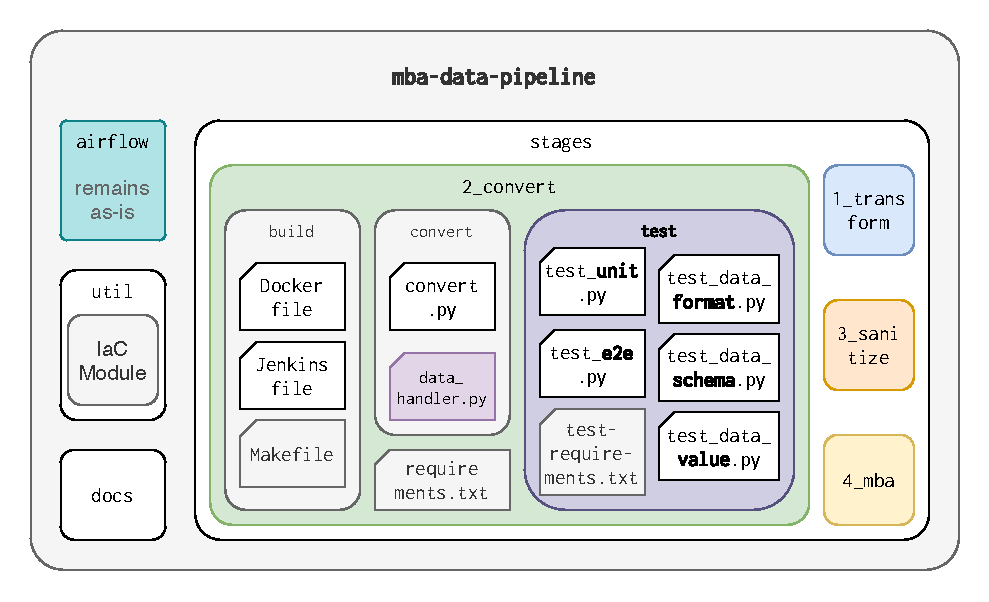
\includegraphics[width=\linewidth]{main-matter/img/5-repo-structure-new}
	\caption{Revisited Project Repository Structure (Testing Included)}
	\label{fig:5-new-repo}
\end{figure}

Figure \ref{fig:5-new-repo} visualizes the testing-enabled repository. Each stage receives its own \texttt{test} directory. This directory contains all testing class files as well as a requirements document, specifying required external installation for testing purposes. This document is similar to the already existing \texttt{requirements.txt} file.

With this change, Jenkins has now got access to the testing classes. Since the current Dockerfile already includes the entire stage module inside the image, the tests can already be run inside virtual Docker containers, which is desired. Currently, Jenkins only holds the production-grade \ac{iam} credentials inside is credential storage. The previously created \ac{iam} testing roles need to be added as well. Finally, the Jenkinsfile can be manipulated in order to provide appropriate testing stages inside the process, resulting in the pipeline depicted in Figure \ref{fig:5-cicd-testing}

\begin{figure}[h!]
	\centering
	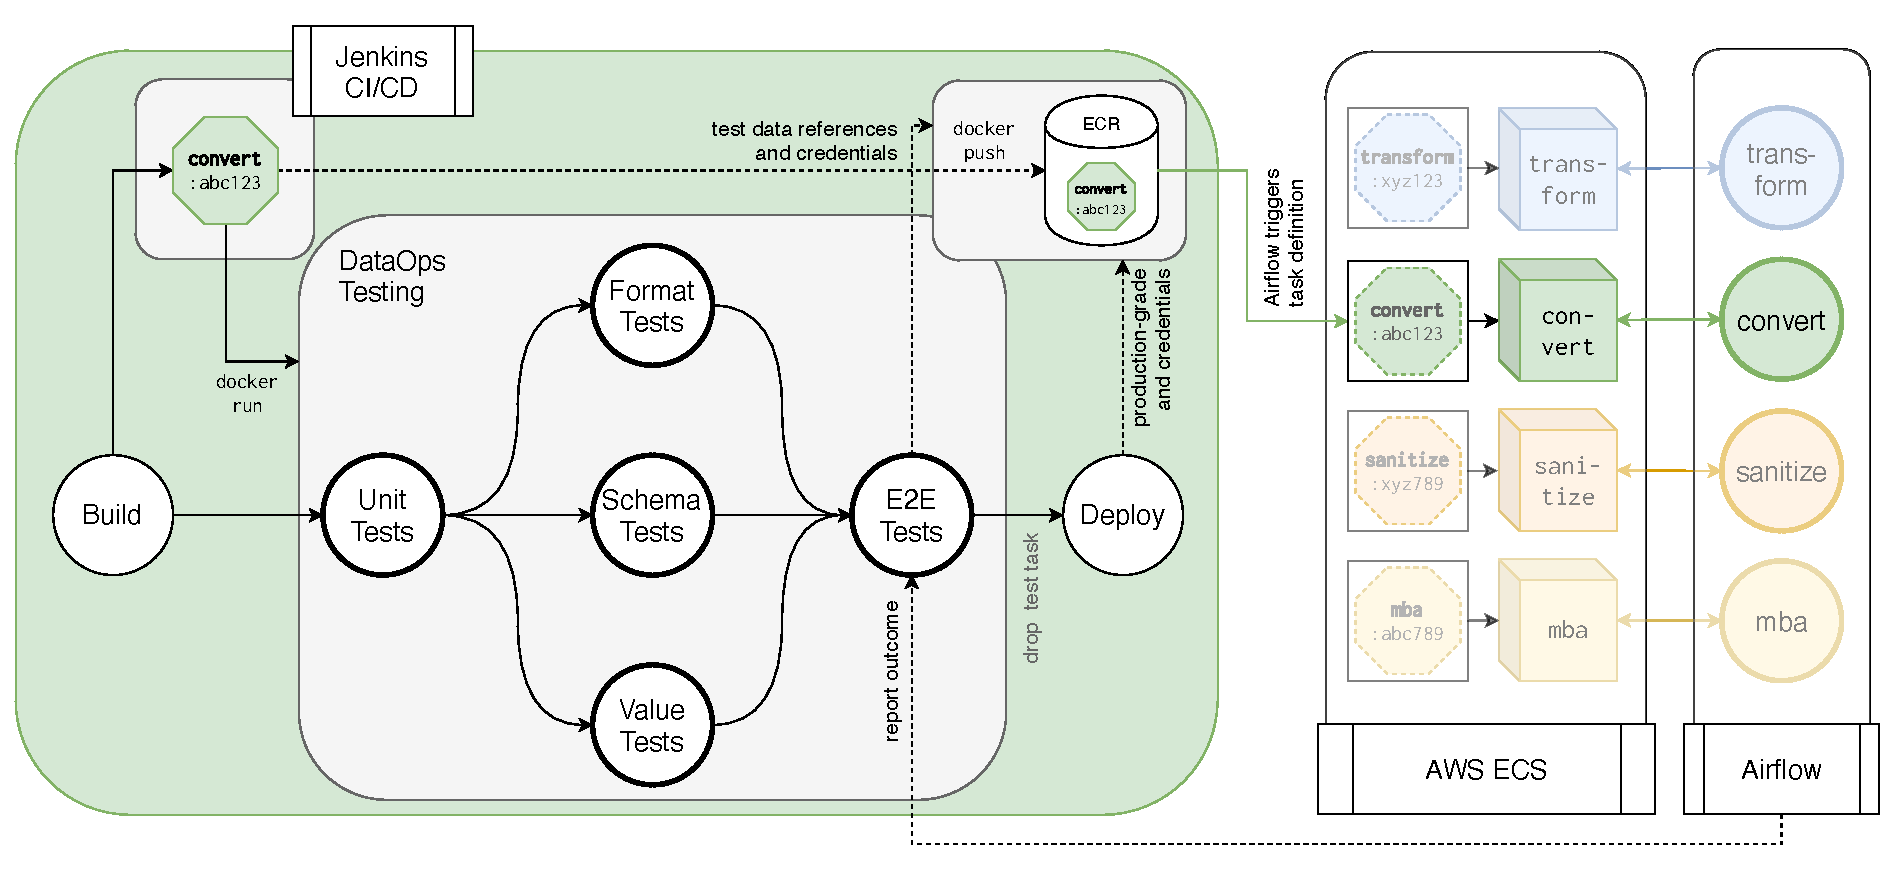
\includegraphics[width=\linewidth]{main-matter/img/5-cicd-testing.pdf}
	\caption{Testing-Enabled \acs{cicd} Pipeline Overview}
	\label{fig:5-cicd-testing}
\end{figure}

The build stage is changed such that the image is built with testing credentials rather than production-grade credentials. Additionally, Jenkins already specifies the test data locations during the image build process. In production, Airflow configures the required data location environment variables inside the task definition. With testing, Jenkins uses the unique Git commit identifier to define the data test job inside the \ac{s3} data lake. Then, testing stages are implemented. Their individual structures are very similar to each other. The testing stages of the Jenkinsfile are specified in Source Code Excerpt \ref{src:5-new-jenkinsfile-test}.

The unit testing stage calls the corresponding unit testing class file (l. 13) when running the Docker container (ll. 9--15). Additionally, a host-to-container volume mount is performed (l. 10) such that Jenkins receives access to the testing report file (l. 14). This file is used to display the testing report inside the Jenkins \ac{ui}. The integration (data) tests are implemented similarly, but run in parallel (l. 24--30). This does not cause any problems since these tests are run in entirely separate containers. The end-to-end test performs a pre-deployment prior to test execution (ll. 35--40). This is required because the test calls the Airflow \acs{api} to execute a test data pipeline including the new version image.

\begin{listing}[h!]
	\inputminted{groovy}{main-matter/src/5-new-jenkinsfile-test}
	\caption{Testing Stages of the Revisited Jenkinsfile}
	\label{src:5-new-jenkinsfile-test}
\end{listing}

Finally, the test deployment is removed and the actual deployment, including production-grade credentials and no data location specification, is performed. The environment changes (i.e., data lake structure and additional \ac{iam} role definitions) are added to the \ac{iac} process of the project. In case of an infrastructure rebuild, these components will be also generated and embedded automatically.

This concludes the implementation task which is now subject to evaluation.


